\documentclass[11pt, a4paper, twoside]{book}

\setlength{\topmargin}{2pt} \setlength{\headheight}{15pt}
\setlength{\headsep}{25pt} \setlength{\textheight}{640pt}
\setlength{\footskip}{25pt}
\setlength{\hoffset}{0pt}
\setlength{\oddsidemargin}{0pt} \setlength{\oddsidemargin}{3pt}
\setlength{\evensidemargin}{0pt} \setlength{\evensidemargin}{30pt}
\setlength{\textwidth}{430pt}
\setlength{\marginparsep}{0pt} \setlength{\marginparwidth}{0pt}

\usepackage[french]{babel}
\usepackage[utf8]{inputenc}
%\usepackage[IT]{fontenc}
\usepackage{graphicx}
\graphicspath{ {images/} }
\usepackage[margin=1.25in]{geometry}

\usepackage{longtable}
\usepackage{float}
\usepackage{textcomp}
\usepackage{amsmath}
\usepackage{pdfpages}

%start of title
{\title{
%include the logo
\begin{figure}[h]
\centering			

\includegraphics[width=0.5\textwidth]{logo}
\end{figure}
ÉCOLE NATIONALE DES SCIENCES APPLIQUÉES DE KÉNITRA \\  \vspace*{1truecm} Moroccan foundation for Advanced Science, Innovation and Research \\ 
(MAScIR) \\
\vspace*{1truecm} Rapport de Projet de Fin d'Année \\ \vspace*{0.5truecm} \textbf{Étude et réalisation d'un system RFID}} 
%end of title

\author{Réalisé par : \\ Otmane BOUAYAD \vspace*{1truecm} \\ Encadré par : \\ Mme Ilham BOUZIDA : Encadrante professionnelle\\ }
\date{(Du 15 Février au 25 Août  2016)}

\begin{document}
\maketitle
\pagestyle{plain}
%Dedicas

\chapter*{Dédicace}

I would like to dedicate this work to my wife, Oumaima, for her love, encouragement, and continuous support,my parents, who has taught me many things in life and include the one thing I’ve tried to live by: 
\emph{“Never give up on your dreams. Hard work and diligence will see you through so long as you never give up.”}
 So it is with all my love, respect, and admiration that I dedicate this to you.My sister and my best friends forever Reda and Nouhaila,my future engineers. remember
\emph{“Accomplishment is product of thoughts, mind is everything”.}

%remerciment
\chapter*{Remerciements}
\addcontentsline{toc}{section}{Remerciements}
\emph{
Avant tout développement sur cette expérience professionnelle, il apparaît opportun 
de commencer ce rapport de stage par des remerciements, à ceux qui nous ont beaucoup 
aidé au cours de ce stage, et même à ceux qui ont eu la gentillesse de faire de ce stage un 
moment très profitable.\\\\}
\emph{
Aussi, Nous tenons plus particulièrement à remercier Mme Ilham
BOUZIDA, ingénieur qualité dans l’équipe packaging à MAScIR, et à M. Brahim LAKSSIR, chef de service packaging à MAScIR,nos maîtres de stage qui ont la part de lion dans notre formation et accompagnement professionnels avec beaucoup de patience et de savoir-faire.\\\\ }
\emph{Je souhaite remercier mon promoteur et mon encadrant à l'école Pr. Tomader MAZRI pour ses instructions et son aide lors du stage.\\\\}
\emph{
Finalement , nous remercions l’ensemble des employés de la Fondation MAScIR pour les conseils qu’ils ont pu nous prodiguer au cours de ce stage.
}\\\\
\emph{Enfin, j’adresse tous mes remerciements les plus sincères à tous les enseignants de l’ENSA de Kenitra pour avoir contribué à la formation que j’ai acquise lors de mon cursus.}
%include the table of content please
\tableofcontents

%include the liste of figure please
\listoffigures

\listoftables

\chapter*{Introduction}
\addcontentsline{toc}{section}{Introduction}
Le terme RFID englobe toutes les techniques qui utilisent les ondes radio pour identifier automatiquement des objets ou des personnes.
Le système RFID autrement dit l'identification par radio fréquence est une technique qui permet de mémoriser et de récupérer des informations à distance grâce à une étiquette qui émet des ondes radio.\\
Le système RFID (audiofréquence identification) est une technique très attractive pour l'entreprise qui offre la possibilité d'une gestion automatique du nombre conséquent d'informations qu'elle doit traiter. Les équipements adaptés à ce système permettent de synchroniser les flux physiques avec les flux d'informations.\\\\
Dans le cadre du projet de fin d'études, j'ai eu l'opportunité de travailler sur cette technique avec la fondation MAScIR qui occupe une position leader sur le marché de la micro-électronique.\\\\
Le projet de fin d’études porte alors, sur l'étude et la réalisation d’une solution RFID UHF qui assure l’identification et la traçabilité des entrées et sorties des palettes. Choisire les tags adaptés aux besoins en respectant les conditions d’utilisation et type de lecteur. Devolopper un logiciel de gestion des palettes. D’autre part, la réalisation d’un transpondeur RFID UHF et une application Android pour gestion du secteur d'agriculture.\\\\
Le mémoire que je présente est organisé en 6 chapitres.

\begin{itemize}
\item Chapitre 1: présentation de l'entreprise d'accueil ainsi qu'une description du déroulement du stage.
\item Chapitre 2: contexte général du Projet.
\item Chapitre 3: étude bibliographique, et principe de fonctionnement d’un système RFID. 
\item CHapitre 4: conception et test de la partie logitiel.
\item Chapitre 5: etude du besoin du secteur agriculture et developement de l'application Android.
\item Chapitre 6: conception d'un transpondeur RFID UHF.
\end{itemize}

\pagestyle{plain}

\chapter{Persentation de l'entreprise d'accueil}
\pagestyle{headings}
\section{Présentation générale de MAScIR}
MAScIR (Moroccan foundation for Advanced Science, Innovation and Research) est un organisme de recherche à caractère scientifique et technologique. Il est voué à la recherche en nanotechnologie, en biotechnologie, en technologie numérique, en microélectronique, en énergie et en environnement, la fondation se veut présenter là où les enjeux de la société l’exigent.\\

La figure suivante montre l’emplacement de l’entreprise.

\begin{figure}[h]
\centering
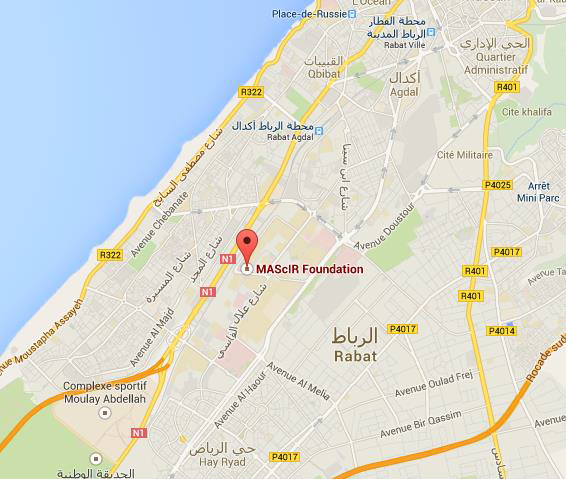
\includegraphics[width=0.75\textwidth]{mascir_map}
\caption{Localisation de la fondation MAScIR}
\end{figure}

Rassemblant d’éminents chercheurs des quatre coins du monde, MAScIR regroupe des équipes scientifiques œuvrant dans des domaines innovants et complémentaires et met à leur disposition une infrastructure scientifique de pointe.\\

Initialement fondée en 2007 par le Gouvernement Marocain en tant que fondation à but non lucratif MAScIR a continué son expansion en créant :

\begin{description}
\item[MAScIR MicroElectronics] a pour objectif de devenir un centre de Recherche et Développement dans le domaine de la microélectronique.
\item[MAScIR BioTechnology] deuxième centre inscrit dans MAScIR œuvrant dans le domaine de la biotechnologie : recherche et développement des médicaments ou des biocides.
\item[NanoTechnology] qui a pour mission de mener des recherches appliquées, innovantes et à la fine pointe de la technologie dans le domaine des nanomatériaux et des nanotechnologies. Ces recherches sont menées par une équipe internationale de haut calibre travaillant dans un environnement unique et utilisant une infrastructure de pointe.
\end{description}

\subsection{Partenaires de la foundation}
Les principaux partenaires de la fondation MASCIR MicroElectronics sont :
\begin{description}
\item[Lear Corporation] est l’un des principaux fournisseurs mondiaux de sièges automobiles et les systèmes de gestion de l’énergie électrique.
\item[Thales] figure parmi les leaders européens de la fabrication et de la commercialisation d'équipements et de systèmes électroniques destinés aux secteurs de l'aérospatial, du transport, de la défense et de la sécurité.
\item[OCP] est un acteur incontournable sur le marché des phosphates et de ses produits dérivés. Présent sur toute la chaine de valeur, il est le premier exportateur de cette matière dans le monde.
\item[COSUMAR] est un groupe marocain, filiale de la Société nationale d'investissement, spécialisé dans l'extraction, le raffinage et le conditionnement du sucre sous différentes formes. Il est devenu l'unique opérateur sucrier marocain après l'acquisition de SUTA, SUCRAFOR, SUNABEL et SURAC en 2005.
\item[STERIMED] est une société spécialisée dans le domaine de l’eau et des technologies de l’environnement. Son objectif est d’accompagner les entreprises et collectivités dans la résolution des problématiques liées à l’eau, l’environnement.
\end{description}

\subsection{Structure et hiérarchie}
La Fondation est gérée par un conseil d’administration qui est investi de pouvoirs de gestion à cet égard. Le Conseil dispose de quatre comités distincts : un Comité d’Investissement, un Comité de suivi, un comité de vérification et un Comité de Rémunération; qui assurent une gestion rapprochée des sujets relatifs à leur mission.
\begin{description}
\item[Conseil d'administration] détermine les orientations stratégiques de MAScIR et veille à leur mise en œuvre dans des réunions régulières. En prenant des décisions, le Conseil compte sur le travail des comités spécialisés.
\item[Comité de vérification] le rôle principal du Comité d'audit est de permettre à la Commission de veiller à la qualité des contrôles internes et l'intégrité de l'information divulguée aux intervenants et aux partenaires.
\item[Comité des Rémunérations] est responsable de faire des recommandations au Conseil sur la nomination des administrateurs. Il est également responsable de l'examen de la politique en matière de rémunération de la haute direction au sein de MAScIR.
\item[Comité de suivi] surveille la mise en œuvre effective et correcte des projets dans le cadre de l'accord signé entre MAScIR et le Gouvernement marocain.
\item[Comité d'Investissement] assiste le Conseil d'administration dans l'accomplissement de sa responsabilité de surveillance pour les actifs d'investissement liés à l'équipement scientifique.
\end{description}

\section{Présentation du département microélectronique}
MAScIR Micro est un centre d’innovation et développement de technologie dans le domaine de la microélectronique. Il se focalise sur la simulation, les tests, le design, le packaging, la qualification et le prototypage des produits microélectroniques.
\subsection{Mission}
Le programme Microélectronique a réuni une équipe de direction de classe mondiale pour assurer la traction initiale sous licence des technologies de pointe qui sont disponibles pour une utilisation immédiate. \\

Le programme Microélectronique a réuni une équipe de direction de classe mondiale pour assurer la traction initiale sous licence des technologies de pointe qui sont disponibles pour une utilisation immédiate. \\

MAScIR Micro fournit des services pour des clients industriels, mais elle développe aussi son propre business dans les domaines suivants :
\begin{itemize}
\item L’intégration et la miniaturisation des systèmes microélectroniques.
\item L’analyse de fiabilité et défaillance des produits.
\item Modélisation des systèmes complexes.
\item Prototypage et industrialisation des produits innovants.
\item Industrialisation des idées et résultats académiques.
\end{itemize}

\subsection{Laboratoires}
Le département microélectronique de MAScIR possède plusieurs laboratoires équipés de technologie avancée :
\begin{itemize}
\item Salle blanche
\item Laboratoire de fiabilité et analyse de défauts
\item Laboratoire électronique
\end{itemize}

\begin{figure}[h!]
\centering
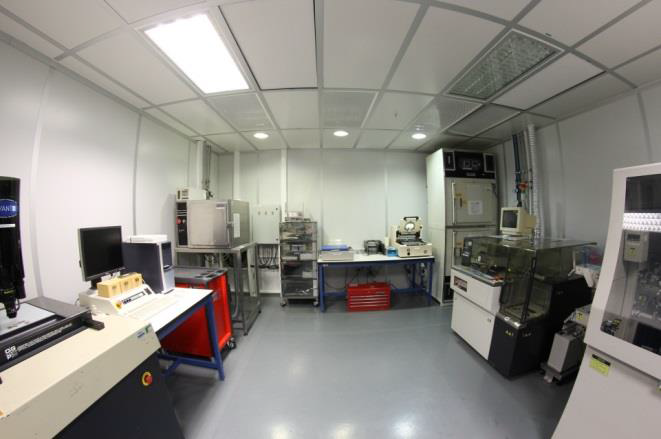
\includegraphics[width=0.75\textwidth]{cleanroom}
\caption{Salle blanche}
\end{figure}

\begin{figure}[h!]
\centering
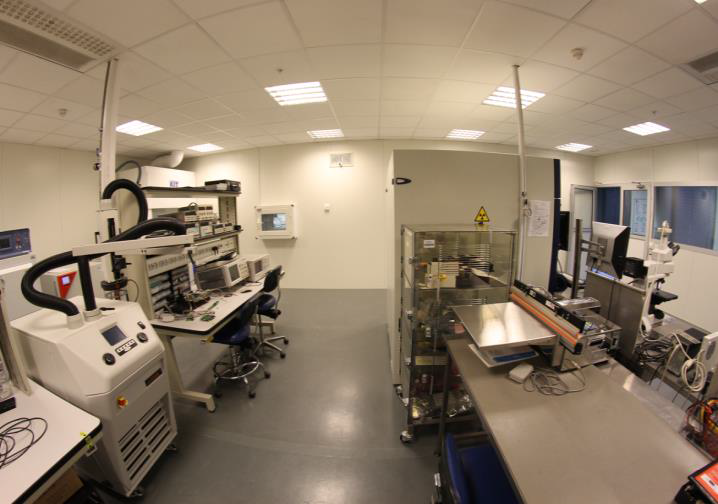
\includegraphics[width=0.75\textwidth]{labo}
\caption{Laboratoire de fiabilité et analyse de défauts}
\end{figure}

\subsection{Équipements}
\begin{itemize}
\item Ligne CSP (Chip Scaled Packaging)
\item Ligne SMT (Surface Mount Technology)
\item SAM (Scanning Accoustic Microscope)
\item X-Ray
\item Chambres climatiques
\end{itemize}

Pour plus d'informations, visiter le site de l'entreprise : \texttt{http://www.mascir.ma}.

\section{Description et déroulement du stage}
\subsection{Activités exercées}
Durant ce stage de fin d’études, j’ai eu l’opportunité de côtoyer le monde industriel et plus précisément de la microélectronique ce qui m’a permis d’assister et participer à plusieurs missions et projets que ce soit au sein de MAScIR ou à l’extérieur.\\

Mis à part le travail sur mon projet, j’ai pu suivre le processus du packaging allant du découpage wafer au marquage boitier et sciage.\\

Parallèlement, J’ai assisté à des manœuvres de vérification de qualité des produits livrés à MAScIR.\\

Par ailleurs, j’ai pu bénéficier d’un encadrement étroit en préparant des réunions pour garantir un bon état d’avancement du projet.

\subsection{Répartition des tâches}
%you need to revise mistakes
\noindent
\textsc{1\textsuperscript{ère} et 2\textsuperscript{ème} semaines :}
\begin{itemize}
\item Visite du local et réunions pour cerner le projet.
\item Bibliographie sur les system RFID.
\end{itemize}
\textsc{3\textsuperscript{ème} et 4\textsuperscript{ème} semaines :}
\begin{itemize}
\item Etude du marcher et choix des tags et lecteur rfid.
\item Participer à la résolution des problèmes du lecteur existant.
\end{itemize}
\textsc{5\textsuperscript{ème} et 6\textsuperscript{ème} semaine :}
\begin{itemize}
\item Etude et familiarisation avec le language \emph{.NET C\#}
\item Realisation d'un prototype de test de lecture de tages.
\end{itemize}
\textsc{7\textsuperscript{ème} et 8\textsuperscript{ème} semaine :}
\begin{itemize}
\item Proposition d'algorithme d'amelioration des performance de la commincation client-lecteur
\item Implementation final du prototype du nouveau protocol de communiation client lecteur.
\end{itemize}
\textsc{9\textsuperscript{ème} semaine :}
\begin{itemize}
\item Developpement d'une interface utilisateur pour le control du flux des donnee et gestion de stockage.
\item Etude du marcher marcaine de l'agrigulture et Etude de besoin .
\end{itemize}
\textsc{10\textsuperscript{ème} et 11\textsuperscript{ème} semaine :}
\begin{itemize}
\item Developpement de la Version une de l'application SmartFlah.
\item Amelioration de la version une de l'application SmartFlah
\end{itemize}
\textsc{12\textsuperscript{ème} et 13\textsuperscript{ème} semaine :}
\begin{itemize}
\item Etude Profondis sur les Tag RFID UHF.
\item Realisation du 1er prototype d'antenne UHF RFID
\end{itemize}
\textsc{14\textsuperscript{ème} et 15\textsuperscript{ème} semaine :}
\begin{itemize}
\item Etude des methode d'optimisation du tailet performance d'antenne.
\item simulation sur CST du 2eme prototype d'antenne
\end{itemize}
\textsc{16\textsuperscript{ème} et 17\textsuperscript{ème} semaine :}
\begin{itemize}
\item simulation sur CST du 3eme prototype d'antenne
\item Redaction du rapport
\end{itemize}



\chapter{Contexte Général du projet}
Le but de ce chapitre est de présenter la problématique du projet, le cahier des charges, la démarche suivie pour répondre au besoin de l’ensemble des parties prenantes du projet et le plan d’action.
\section{Cahier des charges}
\subsection{Objectif}
L’objectif de ce projet est l'étude et la réalisation d’une solution RFID UHF qui assure l’identification et la traçabilité des entrées et sorties des palettes. Choisire les tags adaptés aux besoins en respectant les conditions d’utilisation et type de lecteur et de devolopper un logiciel de gestion des palettes. 
Et comme deuxième axe,la réalisation d’un transpondeur RFID UHF et une application Android pour gestion du secteur d'agriculture qui permet a
l’utilisateur de profiter des fonctions offerte par le système à distance. \\
\subsection{Cachier des charges}
Assurer l’identification et la traçabilité des entrées / sorties palettes
\begin{itemize}
\item Choix des puces/tags adaptés aux besoins (conditions d’utilisation et type de lecteur).
\item Etablir un pgr de gestion des palettes en assurant la traçabilité de leur mouvement.
\item Réalisation et test d’un proto.\\
\end{itemize}
\subsection{Mise au point de la problématique}
Ce projet consiste à développer un système de traçabilité des entrées et sorties des palettes. Trouver les causes racines, choisir les solutions optimales pour un problème ou une situation nécessite une grande compréhension du problème. Dans ce sens, la méthode QQOQCP permet d'avoir des informations élémentaires suffisantes sur toutes les dimensions du problème, pour identifier ses aspects essentiels.\\\\\\\
        
\begin{longtable}{|l|c|}
  \hline
  Quoi & Activité : Développement d’un un système de traçabilité \\
       &  Produit : logiciel de reconnaissance faciale, Application Android, Tag UHF \\
  \hline
  Qui & Division : Client MAcIR\\
  \hline
  Où & MAcIR\\
  \hline
  Quand & Du 15/02/2016 au 15/06/2015\\
  \hline
  Comment & Etat d’art sur les techniques RFID \\
          &  existantes afin de développer un autre plus adapté.\\
  \hline
  Pourquoi & Fournir un système de traçabilité des entrées et sorties des palettes.\\
  \hline
  
\caption{QQOQCP}
\end{longtable}

\section{Deroulement chronologique du stage}
Durant les 4 mois de mon stage, les tˆaches relatives `a mon projet de stage sont organis de la facon suiavante:
\subsection{Etapes	de	réalisaion}
\begin{longtable}{|p{0.35\textwidth}|p{0.2\textwidth}|p{0.2\textwidth}| p{0.15\textwidth}|}
\hline
\textbf{Tâche} & \textbf{Date de début} & \textbf{Date de fin} & \textbf{Durée} \\
\hline
Visites et réunions & 16/02/16 & 18/02/16 & 3 jours \\
\hline
Bibliographie RFID & 15/02/16 & 26/02/16 & 10 jours \\
\hline
Etude du marcher et choix des tags et lecteur rfid & 29/02/16 & 04/03/16 & 5 jours \\
\hline
Participer à la resolution des problemes du lecteur existant.
 & 07/03/16 & 11/03/16 & 5 jours \\
\hline
Etude et familiarisation avec le language \emph{.NET C\#} & 14/03/16 & 18/03/15 & 5 jours \\
\hline
Realisation d'un prototype de test de lecture de tages & 14/03/15 & 25/03/15 & 10 jours \\
\hline
 Etude et proposition d'algorithme pour amelioration des performance de la commincation client-lecteur
 & 28/03/16 & 30/03/16 & 3 jours \\
\hline
Implementation final du prototype du nouveau protocol de communiation client lecteur.
 & 30/03/16 & 10/04/16 & 11 jours \\
\hline
Developpement d'une interface utilisateur pour le control du flux des donnee et gestion de stockage.
 & 11/04/16 & 19/04/16 & 7 jours \\
\hline
Etude du marcher marcaine de l'agrigulture et Etude de besoin & 20/04/16 & 22/04/16 & 3s jours \\
\hline
Developpement de la Version une de l'application SmartFlah. & 20/04/16 & 25/04/16 & 5 jours \\
\hline
Etude Profondis sur les Tag RFID UHF  & 25/04/16 & 28/04/16 & 4 jours \\
\hline
Presenation de MAsIR a SIAM  & 29/04/16 & 29/04/16 & 1 jours \\
\hline
Amelioration de la version une de l'application SmartFlah & 02/05/16 & 04/05/15 & 3 jours \\
\hline
Realisation du 1er prototype d'antenne UHF RFID & 05/05/16 & 13/05/16 & 7 jours \\
\hline
Etude des methode d'optimisation du tailet performance d'antenne. & 16/05/16 & 20/05/16 & 2 jours \\
\hline
simulation sur CST du 2eme et 3eme prototype d'antenne & 23/06/16 & 10/06/16 & 15 jours \\
\hline
Redaction du rapport & 11/06/16 & 15/06/16 & 4 jours \\
\hline
\caption{Répartition des tâches}
\end{longtable}
\subsection{Diagrammes	de	Gantt}
When you write a scientific article, you should lay out your ideas in such a way that your readers can follow them easily. Every new concept should flow directly from the previous material. Yet more often than not, scientific prose can be difficult to understand. What is going on? Readers expect certain pieces of information in certain positions in a sentence. Satisfy these expectations, and your readers will find your writing clear and convincing. Violate them, and your readers will be confused. All readers expect more or less the same things in the same places. And writers commonly violate these expectations. The two most important expectations readers have concern the kind of material that is presented at the beginning of a sentence, in the topic position, and at the end, in the stress position [1]. Here I present my take on how to make the best use of these positions to produce clear and coherent prose.
\section{Décomposition du projet}
Le projet est décomposé principalement en 3 parties :
\begin{itemize}
\item Developpement du Middleware et interface graphique: une partie qui consiste a assurer la communication entre le serveur et le lecteur RFID.
\item Develeppoement de lapplication SmartFlah pour la getion des tag animal.
\item Le transpondeur : la conception du transpondeur UHF RFID de petite taill.\\
\end{itemize}

Chaque partie sera étudiée indépendamment dans les chapitres qui suivent.

\chapter{Etude	détaillée du Projet}
RFID ou identification par fréquence radio, est une technologie en croissance rapide qui a le potentiel de faire de grands impacts économiques sur de nombreuses industries. Bien que la RFID est une technologie relativement ancienne, les progrès les plus récents dans la technologie de fabrication de puces RFID font pratique pour de nouvelles applications et paramètres.\\
Ce chapitre est dédié a l'etude	détaillée de la solution RFID.
\section{Description de la solution}
Cette section présente les bases des systèmes RFID et offre la taxonomie des différents types de systèmes RFID. Nous discutons brièvement deux normes RFID majeures et comment ils se rapportent à la pratique.
\subsection{Le system de base RFID}
La discussion de la technologie RFID a tendance à se concentrer uniquement sur les étiquettes. Il est plus exact de voir RFID comme un système complet qui comprend non seulement des étiquettes, mais aussi d'autres éléments importants. Les systèmes RFID sont constitués d'au moins trois composants principaux:
\begin{itemize}
\item Les étiquettes RFID ou transpondeurs, qui transportent des données d'objet d'identification.
\item Lecteurs RFID, ou des émetteurs-récepteurs, lire et écrire des données dans l'étiquette.
\item Bases de données associés pour l'enregistrements de la donnée d'identification\\
\end{itemize}

Nous illustrons l'interaction de ces composants dans la figure 3.1. Sur cette figure, trois étiquettes sont lisibles par un ou les deux lecteurs, A et B. Par exemple, l'étiquette 1 est lisible que par A, tandis que l'étiquette 2 est lisible par A et B, peut-être en raison de restrictions l'accès. Les lecteurs peuvent alors se connecter à des bases de données avec des enregistrements associés à des données d'identification. Dans ce cas, deux bases de données ont chacun leur propre record.\\
\begin{figure}[h!]
\centering
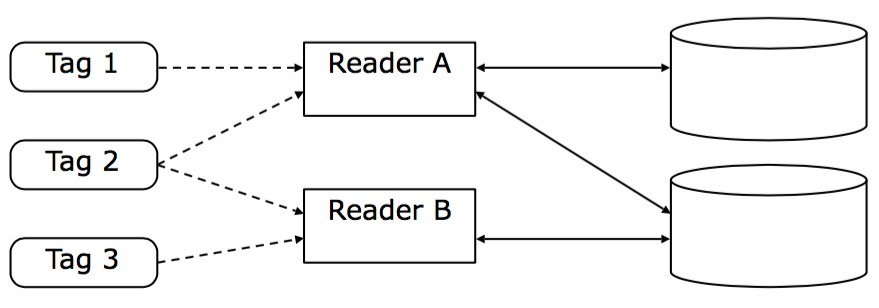
\includegraphics[width=\textwidth]{shema}
\caption{Illustration du système RFID}
\end{figure}
\subsection{Les composants essential d'un system RFID}
\subsubsection{Les tags}
Les tags sont attachés à tous les objets à identifier dans un système RFID. Un tag est généralement
composé d'une antenne ou un élément de couplage, et un circuit intégré. Un important
distinction qui sera discuté plus tard est la source d'alimentation d'un tag. Souvent, les étiquettes ne portent pas une source d'alimentation et doit passivement récolter toute l'énergie d'un signal RF.\\

Il existe plusieurs types de tag qui offrent des fonctionnalités différentes, ont des puissances différentes
de sources ou fonctionnent à des fréquences radio différentes. Chacune de ces variables permet de déterminer
quelles applications une étiquette particulière peut être approprié. Ces différences seront examinées plus loin dans ce chapitre.\\

Les étiquettes modernes ont tendance à mettre en œuvre la fonctionnalité d'identification sur un circuit intégré (IC) qui
assure le calcul et le stockage. Dans le procédé de fabrication, ce circuit intégré est fixé ou
"Attaché" à une antenne avant d'être emballés dans un facteur de forme, comme une capsule de verre ou d'une feuille, qui est intégré dans un produit final.\\
Dans la pratique, les différents fournisseurs effectuent souvent chacune de ces étapes de fabrication. Autres RFID
dessins peuvent être «chipless» ou avoir des informations d'identification au moment de la fabrication, à savoir
"Écriture une fois, lecture nombreuse". \\
\begin{figure}[h!]
\centering
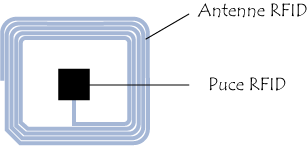
\includegraphics[height=3cm]{tag}
\caption{Tag RFID}
\end{figure}
\subsubsection{Reader/Lecteur}
Les lecteurs RFID communiquent avec des tag à travers un canal RF pour obtenir l'identification
. Selon le type d'étiquette, cette communication peut être un simple ping ou peut être un protocole plus complexe de caractaire multi-tour. Dans les environnements avec de nombreux points, un lecteur peut avoir à effectuer une algorithme d'anti-collision pour veiller à ce que les conflits ne peuvent pas se produire. Les protocoles anti-collision permettent aux lecteurs de communiquer rapidement avec beaucoup de tag en série.

Les lecteurs alimentent souvent ce que l'on appelle les étiquettes passives à travers leur canal de communication RF.
Ces types d'étiquettes ne portent aucune puissance à bord et comptent uniquement sur un lecteur pour fonctionner. Étant donné que ces tag sont si limitées, il compter sur un lecteur pour effectuer des calculs.
Les lecteurs se présentent sous plusieurs formes, fonctionnent sur de nombreuses fréquences différentes, et peuvent offrir un large éventail de fonctionnalités. Les lecteurs peuvent avoir leur propre puissance de traitement et de stockage interne, et peuvent offrir une connectivité réseau. Les lecteurs pourraient être une simple conduit à un système externe, ou pourraient stocker toutes les données pertinentes au niveau local.

À l'heure actuelle, de nombreuses applications reposent sur des dispositifs de lecture fixes. Les premiers essais de EPC à une grande chaîne de supermarchés intégrés dans les lecteurs entrées accueil baies fixes. Ces lecteurs scannent les étiquettes au niveau de la palette que les livraisons de produits arrivent. 

À long terme, les lecteurs peuvent être intégrés à un niveau d'étagère comme une «étagère intelligente». étagères intelligentes seraient scanner pour les balises au niveau de l'article et de surveiller quand ils sont ajoutés et supprimés d'une étagère.

Les lecteurs RFID peuvent également être intégrés dans des appareils mobiles portatifs. Ces lecteurs mobiles permettraient à quelqu'un, par exemple, faire l'inventaire d'un entrepôt en marchant à travers ses allées. Le fabricant de téléphone cellulaire Nokia propose déjà des fonctionnalités RFID de lecture dans certains de leurs téléphones cellulaires [16]. Si les balises de type EPC deviennent très réussie, intéressante et les applications grand public utiles pourraient se poser. Si cela se produit, la fonctionnalité de lecture RFID pourrait devenir une caractéristique commune sur les téléphones, PDA, ou d'autres dispositifs informatiques portables cellulaires
\begin{figure}[h!]
\centering
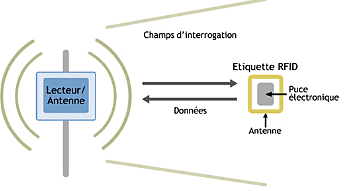
\includegraphics[height=4cm]{reader}
\caption{Interaction du Lecteur RFID avec son environement}
\end{figure}
.\\\\\\\\\\\\\\\\\\\\\\\\\\\\\\\

\subsection{Paires torsadés}
C’est une ligne de transmission formée de deux fils conducteurs enroulés en hélice l’un autour de l’autre, pour maintenir précisément la distance entre les fils et de diminuer la diaphonie.
\begin{figure}[h!]
\centering
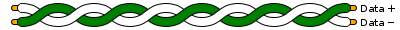
\includegraphics[width=\textwidth]{twistedPair}
\caption{Paires torsadés}
\end{figure}
Elle permet une connexion permanente sans interruption avec un débit qui peut atteindre les 10 Gbits/s. La longueur du câble ne doit pas dépasser 100m, les répétiteurs s'avèrent indispensables si on dépasse cette longueur.
\subsection{Fibre optique}
C'est un fil en verre ou en plastique très fin qui a la propriété d'un conducteur de lumière et sert dans la transmission de données et de lumière.\\

Le fibre optique présente un avantage au niveau de la portée du signal avec un débit très élevé. Son insensibilité au champs électromagnétique lui permet de fonctionner sans problème dans les milieux industriels (présence des moteurs...). Mais, un câble fibre optique contient un cœur très fragile ne lui permettant pas d'être courbé. De plus, son coût élevé présente un majeur point négatif.
\begin{figure}[H]
\centering
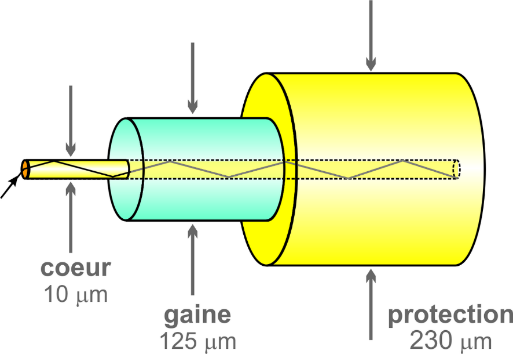
\includegraphics[width=0.4\textwidth]{opticalFibre}
\caption{Fibre optique}
\end{figure}
\subsection{Wifi}
C'est un réseau sans-fil qui relie des appareils informatiques par des ondes électromagnétiques, donc absence de câbles et facilité d'installation avec un coût moins élevé. L'atténuation des signaux avec la présence des obstacles et le problème des interférences provoquent des ruptures de connexions fréquentes donc une instabilité de connexion.
\subsection{Power Line Communication}
C'est une technique de communication qui utilise les câbles du réseau électrique pour transmettre et recevoir les données en mode half-duplex. Il présente une technologique pratique pour des applications sur les smart-grids :
\begin{itemize}
\item Automated meter reading (AMR).
\item Communications SCADA (Supervisory control and data acquisition).
\end{itemize}
\subsection{Tableau Comparative}
Le tableau suivant représente un récapitulatif comparatif entre les différents supports cités dessus suivant les critères suivants :
\begin{longtable}{|p{0.1\textwidth}|p{0.225\textwidth}|p{0.225\textwidth}| p{0.225\textwidth}|p{0.225\textwidth}|}
\hline
 & \textbf{Paires torsadés} & \textbf{Fibre optique} & \textbf{Wifi} & \textbf{Power line Communication} \\
\hline
\textbf{Débit} & Jusqu'à 10Gbits/s & Dépassant le 1Gbits/s & 450Mbits/s & 500Mbits/s \\
\hline
\textbf{Portée} & Câbles \textless 100m & \texttildelow Kms & \texttildelow 140m & \texttildelow Kms \\
\hline
\textbf{Coût} & Moyen & Elevé & Faible & Faible \\
\hline
\textbf{Points forts} & Protocole de communication très connu et facile à implanter & Insensible aux champs électromagnétique & Installation facile & Pas d'installation, développée pour les smart-grids \\
\hline
\textbf{Points faibles} & & Cœur fragile & Interférences, instabilité de connexion & Ne fonctionne pas en triphasé, communication half-duplex \\
\hline
\caption{Tableau comparatif}
\end{longtable}
Après une discussion rigoureuse, le support de communication opté pour ce projet est la communication \textbf{Ethernet (Paires torsadés)}, et \textbf{Power Line Communication (PLC)}.
\section{Power Line Communication (PLC)}
\subsection{Principe}
La technologie PLC consiste à superposer au signal électrique (50Hz), un 2ème signal à plus haute fréquence (de 1KHz à des MHz) et de faible énergie, ce signal se propage sur l'installation électrique et qui peut être reçu et décodé à distance.
\begin{figure}[H]
\centering
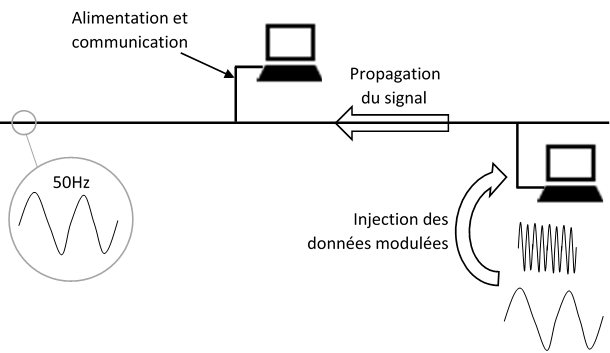
\includegraphics[width=\textwidth]{PLC}
\caption{Principe du PLC}
\end{figure}
Pour faire communiquer deux équipements par un réseau PLC, il faut que chaque dispositif dispose d’un modulateur/démodulateur et un circuit de couplage et d'injection du signal dans le réseau.
\subsection{Caractéristique du Modulateur/Démodulateur choisi}
Le modulateur choisi est ST7538Q du fabriquant ST Microelectronics, c'est un modem FSK
\footnotemark \ qui fonctionne en mode Half Duplex, il est conçu pour les applications PLC. Il est commandé par une interface série synchrone ou asynchrone.\\

\footnotetext{Frequency-Shift Keying}
\begin{figure}[h]
\centering
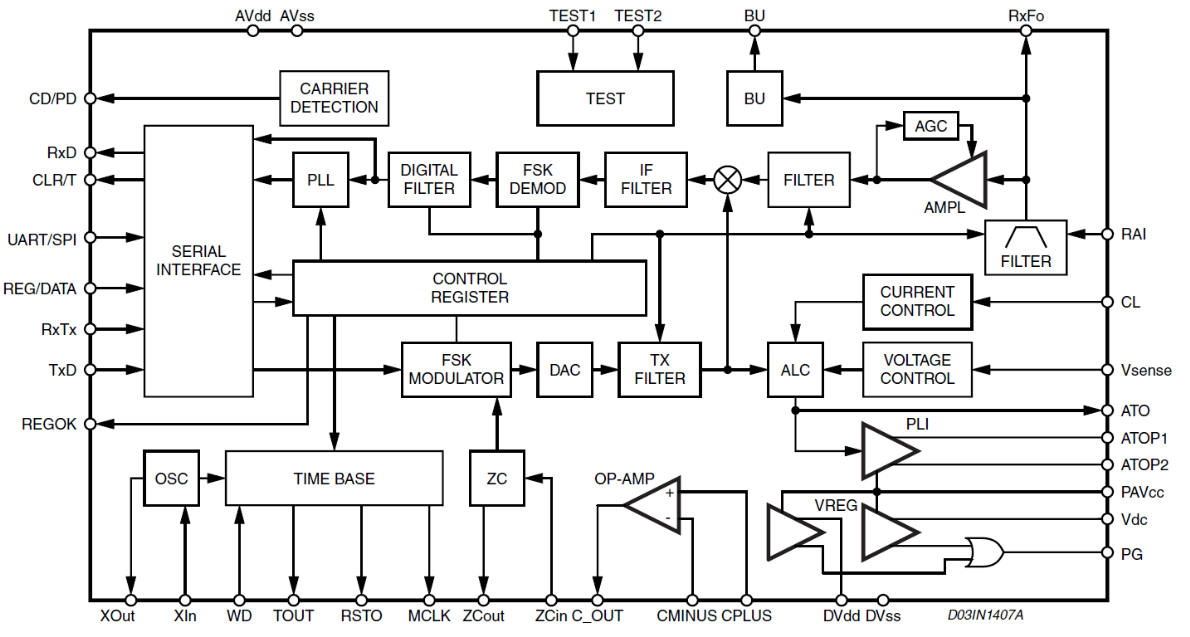
\includegraphics[width=\textwidth]{st7538Q}
\caption{Diagramme de ST7538Q}
\end{figure}
Ses principales caractéristiques sont :
\begin{itemize}
\item Modulation par déplacement de fréquence (FSK) Half duplex.
\item Une seule tension alimentation (entre 7.5V et 12.5V).
\item Consommation très faible (5mA).
\item 8 fréquences de modulation programmables.
\item Vitesse de transmission allant jusqu’à 4800B/s.
\item Sensibilité de réception jusqu’à 250 µVrms.
\item Conforme avec la norme EN 50065 CENELEC.
\item CSMA/CA\footnotemark.
\item Compatible avec les interfaces UART et SPI.
\end{itemize}
\footnotetext{Carrier Sense Multiple Access (Collision Avoidance)}

Dans ce projet, on utilisera la fréquence porteuse maximale (132.5KHz) avec une vitesse de transmission de 4800B/s et une déviation de 1.
\begin{equation}
\Delta f=Baud \cdot Deviation = 4.8 KHz
\end{equation}
Les fréquences mark et space utilisées sont défini par les formules suivantes :
\begin{equation}
F(0) = f + \dfrac{\Delta f}{2} = 134.9KHz
\end{equation}
\begin{equation}
F(1) = f - \dfrac{\Delta f}{2} = 130.1KHz
\end{equation}
\begin{center}
\textbf{\emph{Note :}}\\
\emph{Pour plus d'informations sur les fréquences et les débits supportées par ST7538Q consulter son datasheet.}
\end{center}
\subsection{Méthode d’accès à ST7538Q}
Ce modulateur échange les données avec le microcontrôleur à travers une des deux communications séries :
\begin{itemize}
\item Synchrone à l'aide du protocole SPI
\item Asynchrone à l'aide du protocole UART
\end{itemize}
Les pins \texttt{RxD} et \texttt{TxD} sont pour recevoir et envoyer respectivement les documents du microcontrôleur vers le modem.
\texttt{RxTx} est pour spécifier si on est en mode réception(1) ou transmission(0),
\texttt{REG\_ DATA} est pour spécifier si les données vont être modulées et injecté ou une configuration de registre, finalement, \texttt{CLR/T} est le signal d'horloge imposé par le modem dans le mode synchrone.
\\

\begin{figure}[h]
\centering
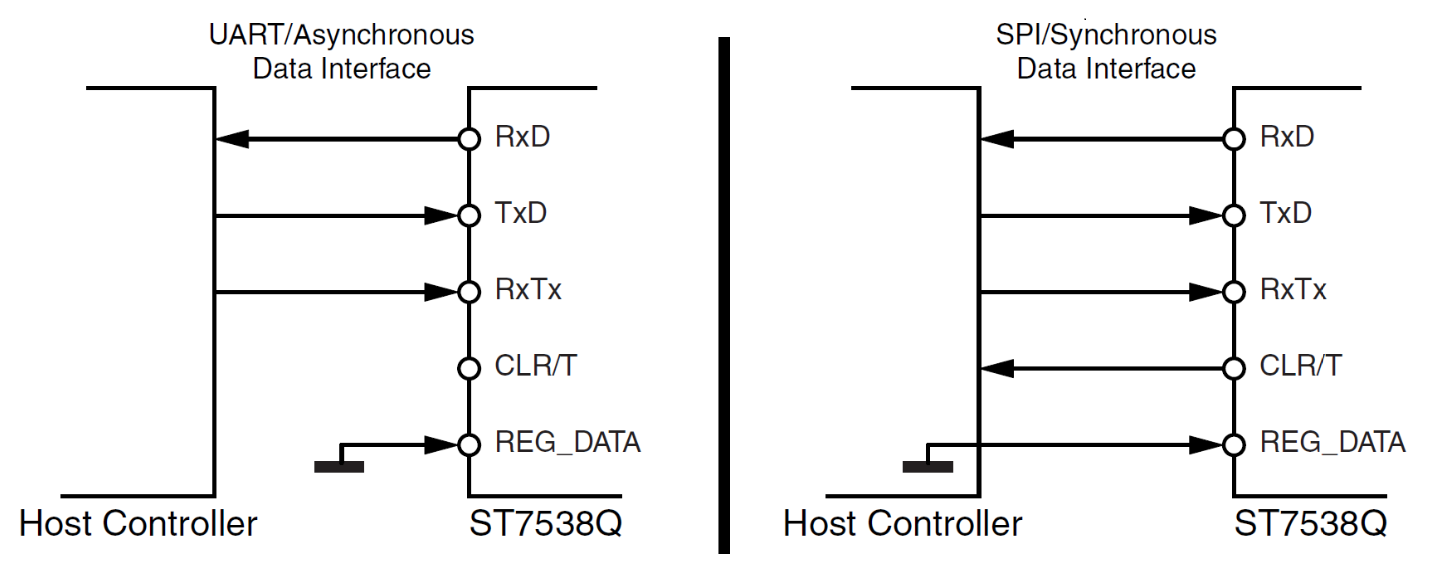
\includegraphics[width=\textwidth]{interfSt7538Q}
\caption{Interface synchrone et asynchrone entre Microcontrôleur et ST7538Q}
\end{figure}
Le protocole utilisé dans ce projet est la communication asynchrone moyennant l'UART.
\subsection{Circuit de couplage et d’injection}
Le circuit de couplage lie le modulateur avec la ligne pour transmettre et recevoir le signal modulé efficacement, et il contient un système de filtrage de la tension de réseau (220V\texttildelow 50Hz ou 110V\texttildelow 60Hz) et les bruits qui vont surgir lors du transfert.
\begin{figure}[h]
\centering
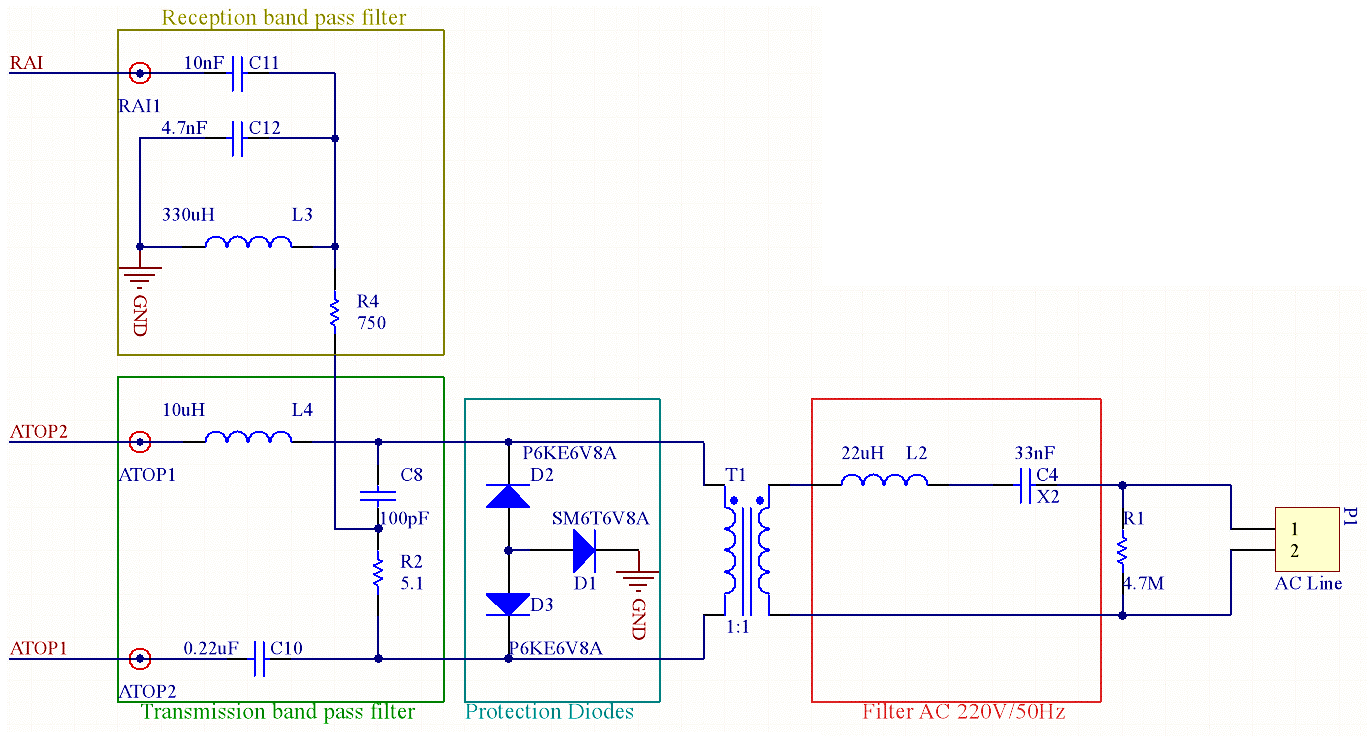
\includegraphics[width=\textwidth]{couplingCircuit}
\caption{Circuit de couplage}
\end{figure}
\\

Il est possible de mettre en œuvre différentes topologies de circuits de couplage. Une première classification est comprise entre une solution isolée avec un transformateur de ligne ou une double capacité et une solution non isolé avec un seul condensateur de découplage à haute tension. La dernière est plus simple et plus économique, tandis que la première permet d'obtenir de meilleures performances en utilisant efficacement la puissance de sortie différentiel des dispositifs.\\

La solution de différentiel a été également plus pratique pour l'avantage pour réduire les harmoniques paires des signaux transmis.\\

La solution implémentée est conforme à la norme \textsc{cerelec - en 50065-1}, il est composé d’un circuit isolé avec un transformateur 1:1 et une capacité de class X2\footnotemark \ pour éliminer la fréquence 50Hz (220V). Le circuit de transmission n'a aucune influence sur le circuit de réception, donc les deux structures peuvent être analysées séparément. Les filtres sont dimensionnés pour la fréquence 132.5 kHz et pour avoir une communication fiable.
\footnotetext{Une capacité conçue pour opérer entre la phase et le neutre (200V-240V)}
\subsubsection{Partie de transmission}
La fonction du circuit de transmission et d'injecter le signal sortant de l'amplificateur de puissance (\texttt{ATOP1}/\texttt{ATOP2}) du modem dans le réseau électrique avec une efficacité maximale en filtrant les bruit suivant la norme \textsc{cenelec} ({\textsc{en}50065-1, \textsc{section 7 : disturbances limits}).\\

Le filtre utilisé dans la transmission est un filtre de 4\textsuperscript{ème} ordre (4 pôles et 2 zeros). Pour avoir une bonne bonne distribution d'échauffement et une insensibilité à la variation de la charge, le filtre a une bande de 60kHz (voir figure \ref{fig:filterCharacteristic}). Pour avoir cette caractéristique les deux pôle vont être mis dans les deux fréquences 100kHz et 160kHz.\\

Pour un dimensionnement correcte, l'influence entre les composants doit être prise en considération : L'inductance de fuite du transformateur (de 0.1µH à 10µH), la capacité interne du diode Transil (presque 2nF), la résistance équivalente en série des capacités et bobines (entre 100m$\Omega$ et 1$\Omega$).\\

De plus il faut prendre en considération les impédances existant dans le réseau électrique, le réseau artificiel \textsc{cispr16-1} :
\begin{figure}[H]
\centering
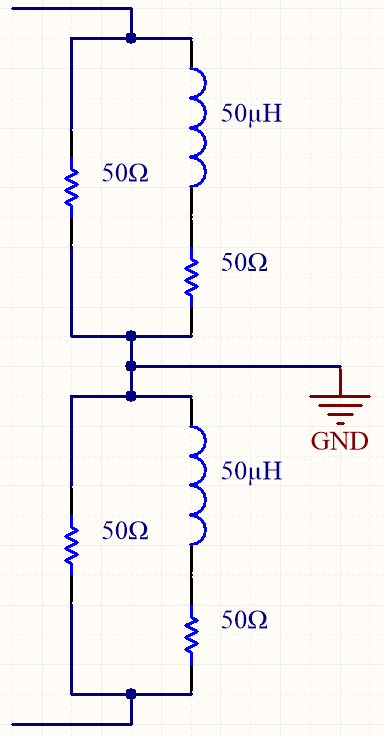
\includegraphics[width=0.25\textwidth]{cispr}
\caption{Réseau artificiel \textsc{cispr16-1}}
\end{figure}
Pour une première approximation des valeurs des composants, on considérera que les parties réactives, et que le transformateur T1 est idéal :
\begin{figure}[H]
\centering
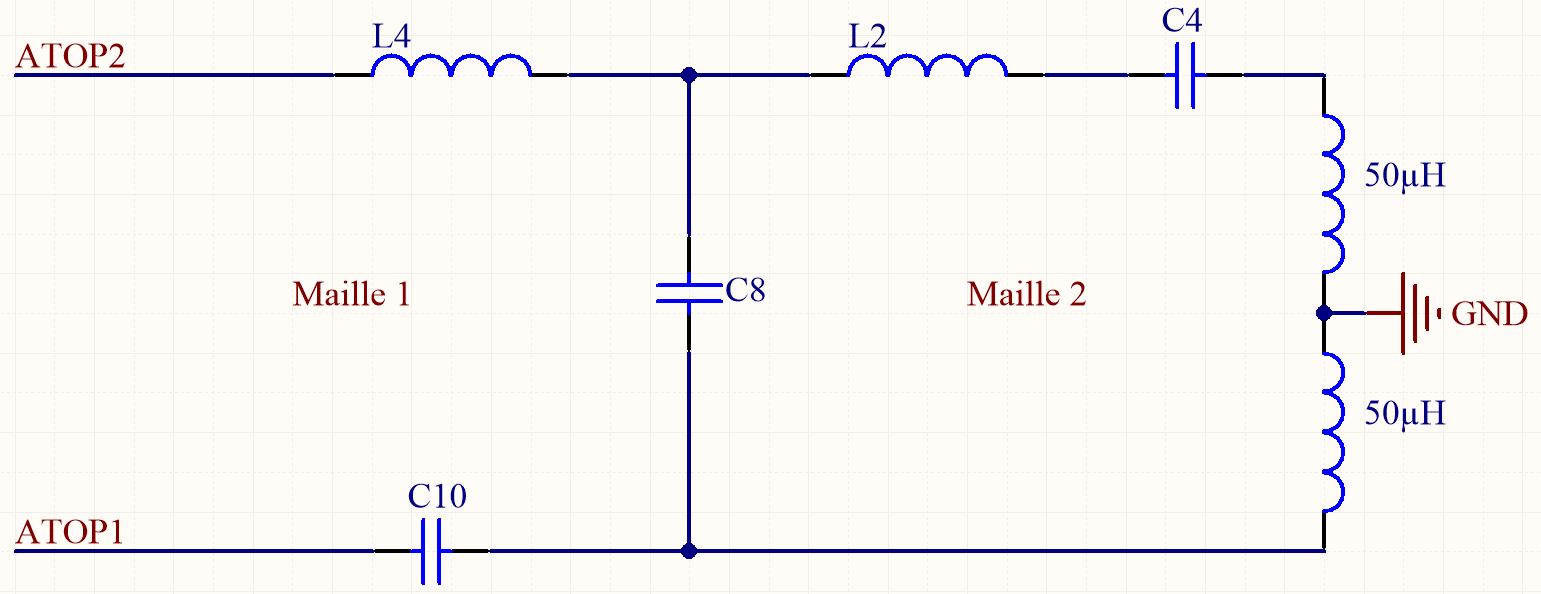
\includegraphics[width=\textwidth]{simplifiedTransmission}
\caption{Schéma simplifié du filtre de transmission}
\end{figure}
Les formules des quatre pôles est données par :
\begin{equation}
\label{equ:pole12}
f_{p1}=f_{p2}\cong \dfrac{1}{2\pi \cdot \sqrt{L_4\cdot C_A}}\cong 160kHz
\end{equation}
\begin{equation}
\label{equ:pole34}
f_{p3}=f_{p4}\cong \dfrac{1}{2\pi \cdot \sqrt{L_B\cdot C_B}}\cong 160kHz
\end{equation}
\begin{center}
avec : $\dfrac{1}{C_A}=\dfrac{1}{C_8}+\dfrac{1}{C_{10}}$;
$\dfrac{1}{C_B}=\dfrac{1}{C_8}+\dfrac{1}{C_4}$
\end{center}
Pour que l'ESR\footnotemark \ des bobines soit le plus faible, que leurs inductances soit faible aussi (\textbf{$L_4$=10µH et $L_2$=22µH}).
\footnotetext{Equivalent series resistance : Résistance équivalente en série}
\\

Une autre contrainte concerne la capacité $C_4$. Il est une capacité de classe X2 qui a une fonction principale de découpler le transformateur du réseau électrique.  Il est préférable que sa valeur soit la plus faible possible pour des raisons économique, tout en gardant le courant de la fréquence 50Hz très faible pour éviter la saturation du transformateur. La valeur choisi est \textbf{33nF}. Donc le courant passant par le transformateur est d'ordre de :
\begin{equation}
|I_{rms}|\cong 220V_{rms}\cdot 2\pi \cdot 50Hz\cdot C_4=2.3mA_{rms}
\end{equation}
Après ces suppositions et en utilisant les équations \ref{equ:pole12} et \ref{equ:pole34}, on obtient \textbf{$C_8$=100nF} et \textbf{$C_{10}$=220nF}.
La résistance $R_2$ est ajouté pour ajuster l'impédance de sortie du filtre de réception.
\begin{figure}[H]
\label{fig:filterCharacteristic}
\centering
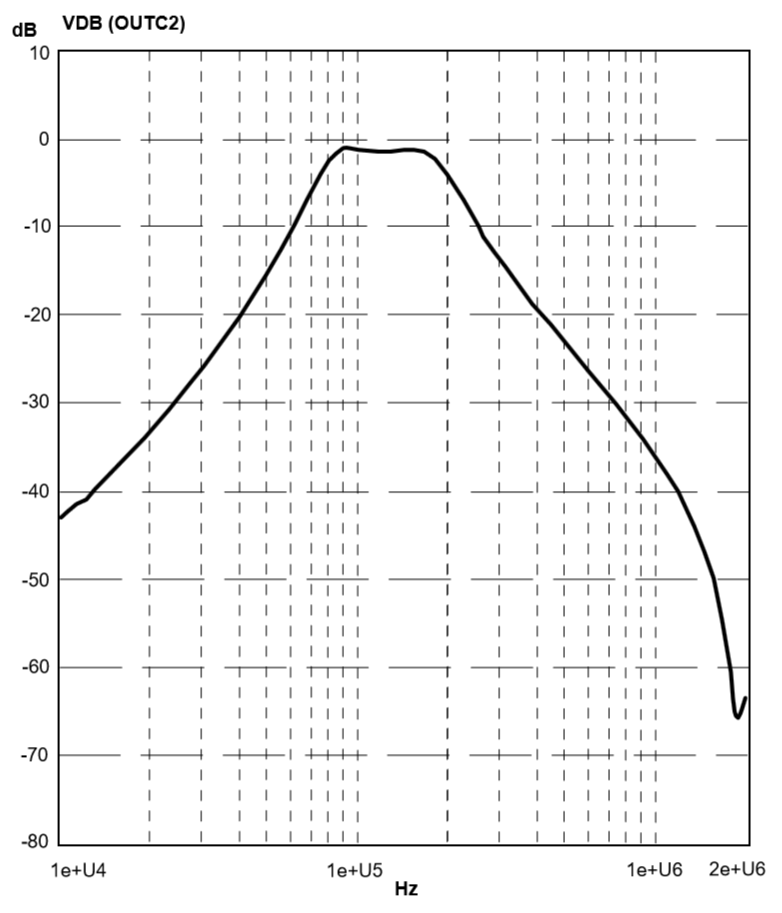
\includegraphics[width=\textwidth]{filterCharacteristic}
\caption{Fonction caractéristique du filtre de transmission}
\end{figure}

\subsubsection{Partie de réception}
Le filtre de réception a pour but de filtrer les bruit venant du réseau qui peuvent dépasser les grandeurs maximales supportés par l'entrée \texttt{RAI}, ou dégrader les performances de démodulation (\textsc{en50065-2-1, section 7.2.3: narrow-band conducted interference}).\\

La solution adopté est un filtre passif de second ordre ($C_{12}$, $L_3$, $R_4$), $C_{11}$ est une capacité de découplage.\\

En mode de réception, la sortie \texttt{ATOP1} est en haute impédance tandis que la sortie \texttt{ATOP2} est lié à la masse (avec une résistance de quelque milliohm). Avec cette configuration, $L_2$, $C_4$, $L_4$, $C_8$ et $R_2$ peuvent être négligés.
Avec ces hypothèses, le dimensionnement du filtre de réception dépend principalement de $C_{12}$, $L_3$ et $R_4$, qui constitue un filtre passe-bande de second ordre d'une fréquence de :
\begin{equation}
\label{equ:recevingFilter}
f_0\cong \dfrac{1}{2\pi \cdot \sqrt{L_3\cdot C_{13}}}=132.5kHz
\end{equation}
Un autre paramètre à prendre en considération est le facteur de qualité(Q) qui doit être le plus grand possible :
\begin{equation}
\label{equ:qualityFactor}
Q\cong R_4\cdot \sqrt{\dfrac{C_{12}}{L_3}}
\end{equation}
Pour ne pas influencer la partie de transmission et de réduire le courant qui va parcourir le transformateur, la valeur de $R_4$ doit être assez grande sans qu'elle participe à l'augmentation du bruit blanc. la valeur \textbf{750$\Omega$} satisfait ces deux conditions. En fixant cette résistance en peux facilement déduire les valeur de $C_{12}$ et $L_3$ à partir des deux équations \ref{equ:recevingFilter} et \ref{equ:qualityFactor}:
\begin{center}
\textbf{$C_{12}$=4.7nF} et \textbf{$L_3$=330µH}
\end{center}
\section{Ethernet}
Physiquement, les composants qui participant à la communication Ethernet sont : Le processeur, Contrôle d'accès au support\footnotemark \ et le PHY chip.
\footnotetext{Media Access Control en anglais ou MAC}
\subsection{Contrôle d'accès au support}
C'est la moitié basse de la couche liaison de données du modèle OSI, elle sert d'interface entre la partie logicielle contrôlant la liaison d'un nœud (Contrôle de liaison logique) et la couche physique. Le rôle de la sous-couche MAC est principalement de :
\begin{itemize}
\item reconnaître le début et la fin des trames dans le flux binaire reçu de la couche physique ;
\item délimiter les trames envoyées en insérant des informations (comme des bits supplémentaires) dans ou entre celles-ci, afin que leur destinataire puisse en déterminer le début et la fin ;
\item détecter les erreurs de transmission, par exemple à l'aide d'une somme de contrôle (checksum) insérée par l'émetteur et vérifiée par le récepteur ;
\item insérer les adresses MAC de source et de destination dans chaque trame transmise ;
\item filtrer les trames reçues en ne gardant que celles qui lui sont destinées, en vérifiant leur adresse MAC de destination ;
\item contrôler l'accès au média physique lorsque celui-ci est partagé.
\end{itemize}
\subsection{PHY chip}
C'est un composant qui opère dans la couche physique du modèle OSI. Techniquement, Le PHY est un circuit intégré qui envoi et reçoit les trames Ethernet, il est l'interface entre le domaine analogique de la modulation en ligne et le domaine numérique. Souvent on trouve que le MAC et le PHY sont groupé dans un seul circuit intégré comme le cas \texttt{DP83816} de Texas Instrument.
\begin{center}
\textbf{\emph{Note :}}\\
\emph{Dans ce projet le composant MAC/PHY est intégré dans le microcôntroleur choisi, et il sera discuté dans le paragraphe \ref{sec:ethernet}}.
\end{center}

\chapter{La partie commande}
Dans ce chapitre, on s'intéresse à la conception de la partie commande du micro-onduleur pour pouvoir intégrer la partie communication efficacement.
\section{Micro-onduleur}
Le micro-onduleur est un onduleur qui fonctionne avec un seul panneau photovoltaïque, il convert le courant issue de ce dernier et le convertit en sinusoïdale de fréquence 50Hz ou 60Hz pour un but d'alimentation, stockage ou injection dans le réseau électrique.\\

Les micro-onduleurs ont plusieurs avantages sur les onduleurs classiques. Le principal avantage est que la présence de petites quantités d'ombrage, de débris ou de neige sur une quelconque module solaire, ou même un échec complet pour le module, ne réduisent pas de façon disproportionnée la sortie de l'ensemble du réseau. Chaque micro-onduleur récolte la puissance optimale en effectuant le suivi du point de puissance maximale(MPPT) pour son module connecté.
\begin{figure}[H]
\centering
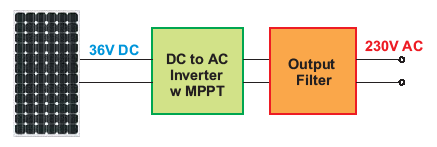
\includegraphics[width=0.8\textwidth]{microinverter}
\caption{Structure d'un micro-onduleur}
\end{figure}

\section{Architecture existante}
\begin{figure}[h]
\centering
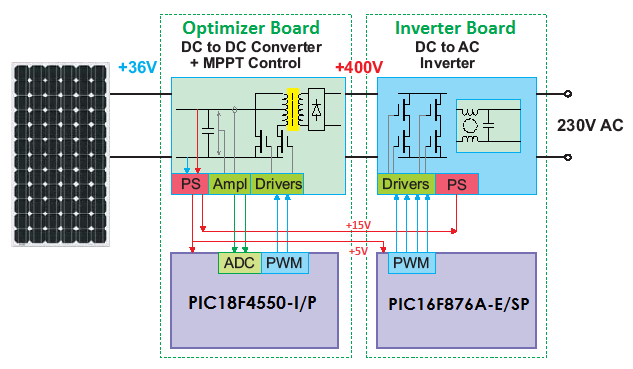
\includegraphics[width=0.85\textwidth]{existingMicroinverter}
\caption{Structure du micro-onduleur existante}
\end{figure}
Le micro-onduleur existant est composé de deux parties, chacune des parties est réalisé dans un circuit imprimé(PCB).\\

La première partie est l'optimiseur. Elle composé de deux hacheurs élévateurs de tension en parallèle qui sont commandé par un signal PWM venant du microcontrôleur PIC18 à travers des Drivers. Ce microcontrôleur fait aussi une lecture de tension et courant généré par le panneau photovoltaïque pour pouvoir exécuter l'algorithme MPPT. Elle contient aussi des régulateur à l'entrée pour extraire une tension pour alimenter le microcontrôleur(5V) et une autre pour commander les MOSFETs(15V).\\

La deuxième partie contient un pont en H pour générer une ondulation commandé par un deuxième microcontrôleur PIC16 à travers des Drivers.
\section{Architecture proposée}
\begin{figure}[h]
\centering
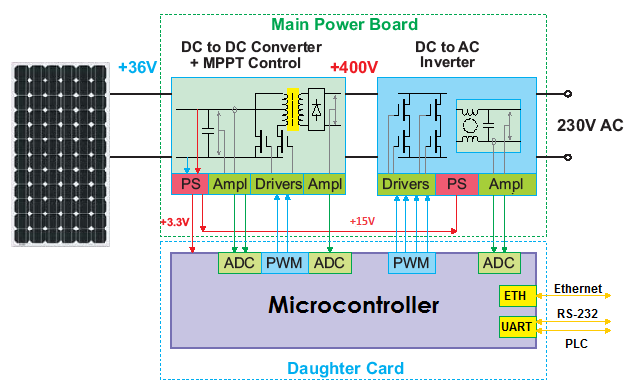
\includegraphics[width=0.85\textwidth]{newMicroinverter}
\caption{Structure du micro-onduleur proposé}
\end{figure}
Pour ajouter la partie communication au micro-onduleur, il faut un microcontrôleur capable de communiquer en utilisant les deux supports de communication cité précédemment, Or l'existence de deux unités de commande rend l'appareil encombrante et plus coûteuse, sachant bien que la tâche fournit ne demande pas trop de calcul. Pour cela une seule unité de commande s'occupant de ces tâche est préférable.\\

La partie puissance est implanté dans un seul circuit imprimé, alors que la partie commande et la partie communication sont implanté dans un seul circuit imprimé appelé Carte-fille, cela donnera une flexibilité pour un futur changement(Par exemple changement de support de communication, ajout d'un écran...).\\
Cette solution fait appel à plus de convertisseur analogique numérique(ADC). Ils vont être utilisé pour faire une lecture du courant et tension à l'entrée de l'optimiseur, déduisant ainsi la puissance produite par le panneau solaire. La lecture de la tension à la sortie de l'optimiseur sera utile pour maintenir la tension de sortie à 220V. La lecture de la tension et le courant à la sortie de l'onduleur permettra de calculer la puissance fournie.
\section{Choix du microcontrôleur}
La topologie proposé précédemment et les supports de communications choisis nous indique les critère suivantes :
\begin{itemize}
\item Avoir un module PWM de 6 canaux, et d'être compatible avec un DMA de préférence.
\item Un convertisseur analogique numérique de 5 canaux.
\item Deux module d'UART.
\item Un module d'Ethernet.
\end{itemize}
Après une étude détaillé, le microcontrôleur adapté à ces contraintes est MCF52230 d'architecture Coldfire V2 de Freescale. Il est principalement caractérisé par :
\begin{itemize}
\item Noyau Coldfire V2 avec 56 MIPS @ 60MHz en exécutant à partir de la mémoire Flash interne.
\item Fast Ethernet Controller(FEC)
\item Ethernet Transceiver(EPHY)
\item Trois universal asynchronous/synchronous receiver/transmitters(UARTs)
\item 8 canaux de 12bits d'ADC
\item 4 canaux de direct memory access(DMA)
\item 8/4 canaux de 8/16 bits PWM
\end{itemize}
\subsection{Ethernet}
Ce microcontrôleur dispose d'un Fast Ethernet Controller(FEC) qui s'occupe de la communication avec le protocole Ethernet. Ce module utilise les broches suivantes :
\begin{itemize}
\item \texttt{PHY\_RXN} et \texttt{PHY\_RXP} pour la réception.
\item \texttt{PHY\_TXN} et \texttt{PHY\_TXP} pour la transmission.
\item \texttt{PHY\_VDDA}, \texttt{PHY\_VDDTX} et \texttt{PHY\_VDDRX} pour l'alimentation, ils ont lié à la masse à travers une capacité de découplage de 100nF.
\item \texttt{PHY\_RBIAS} pour une tension de référencement, doit être lié à une résistance lié à la masse de 12.4k$\Omega$ 1\%.
\item \texttt{PHY\_VSSA}, \texttt{PHY\_VSSTX} et \texttt{PHY\_VSSRX} lié directement à la masse.
\item \texttt{PHY\_ACT} et \texttt{PHY\_LNK} pour commander les LEDs d'activité et de connexion.
\end{itemize}

\begin{figure}[h]
\centering
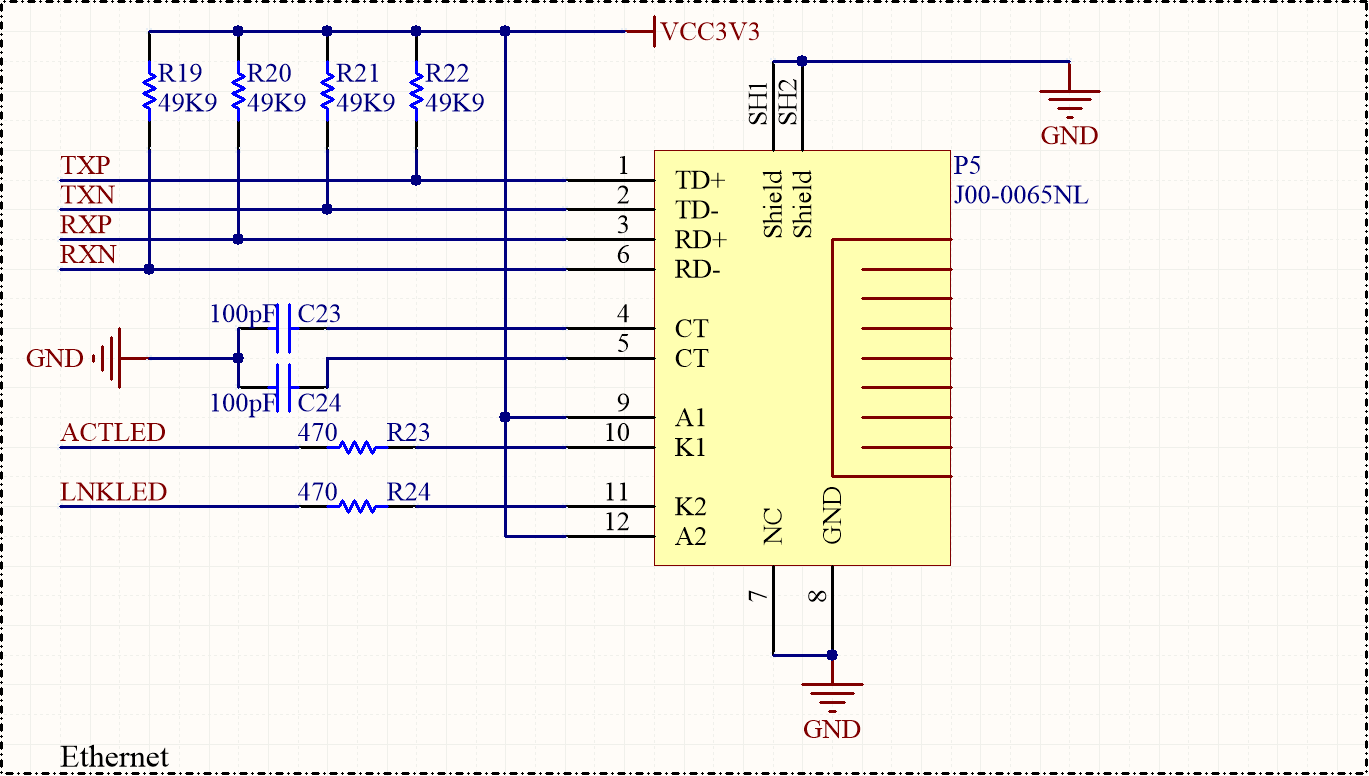
\includegraphics[width=\textwidth]{ethernet}
\caption{La connexion du connecteur RJ-45}
\end{figure}
Les broches \texttt{PHY\_RXN}, \texttt{PHY\_RXP}, \texttt{PHY\_TXN} et \texttt{PHY\_TXP} sont connecté aux \texttt{RD-}, \texttt{RD+}, \texttt{TD-} et \texttt{TD+} respectivement avec une résistance de rappel d'une valeur de 49.9k$\Omega$.
Les résistances $R_{23}$ et $R_{24}$ limite le courant pour les LEDs. Le connecteur RJ-45 inclue des transformateurs de d'isolement.
\label{sec:ethernet}
\subsection{RS-232}
Le schéma de la communication RS-232 est assez simple, il fait appel à un circuit intégré qui fait la conversion de 3.3V issue du microcontrôleur à $\pm$12V et inversement.
\begin{figure}[h]
\centering
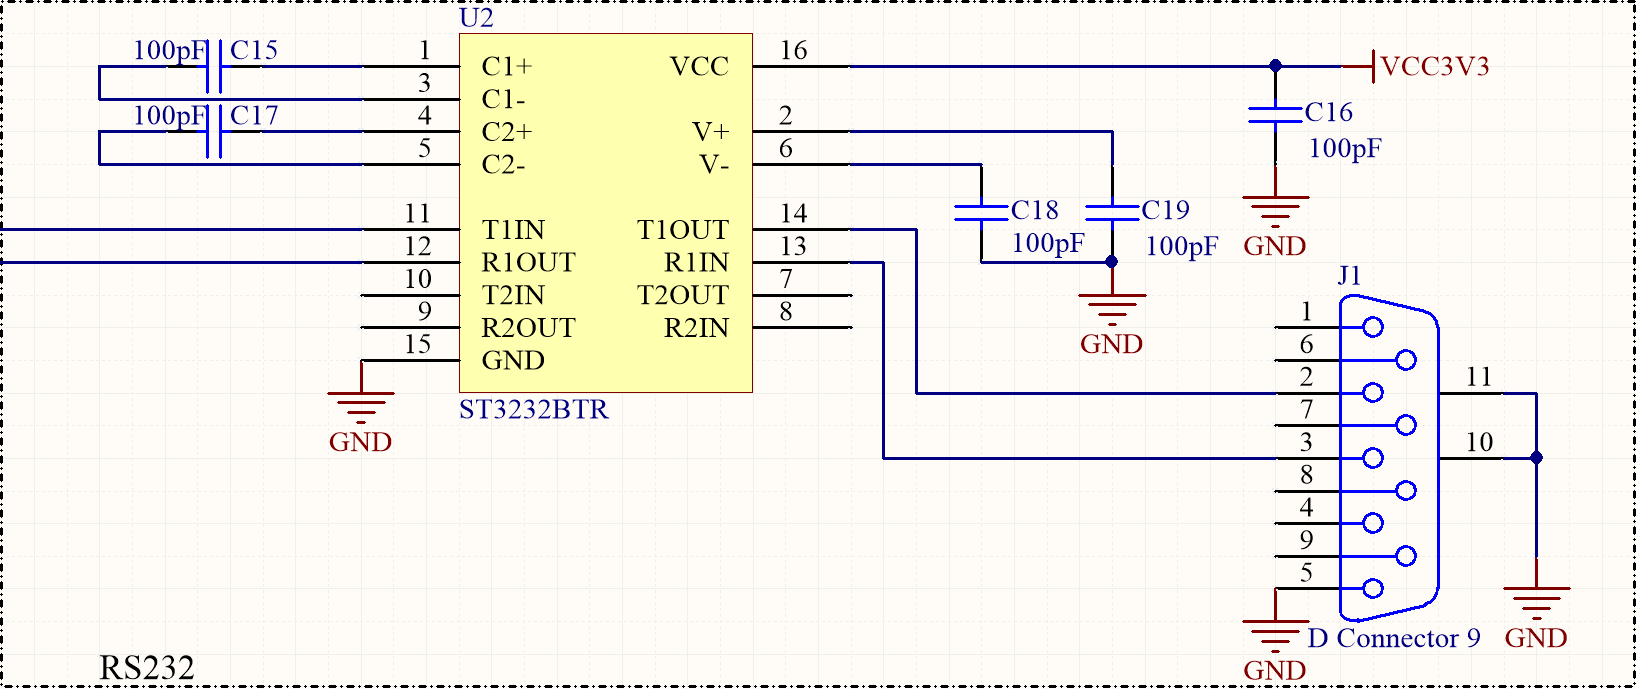
\includegraphics[width=\textwidth]{rs232}
\caption{La communication RS-232}
\end{figure}

\chapter{Algorithme et implantation}
Ce chapitre va cerner le programme avec toute ses parties (algorithme, système d'exploitation...) qui sera implanté dans le microcontrôleur.
\section{Système d'exploitation MQX}
Freescale MQX est un système d'exploitation temps réel (RTOS) qui offre des performances en temps réel dans des microcontrôleurs de taille petite. Il est très intégré avec les derniers microcontrôleurs 32bit de Freescale.\\

MQX est conçu pour avoir une architecture microkernel basé sur des blocs, permettant ainsi une personnalisation des options, de la taille et la vitesse en activant seulement les blocs voulu.
\begin{figure}[H]
\centering
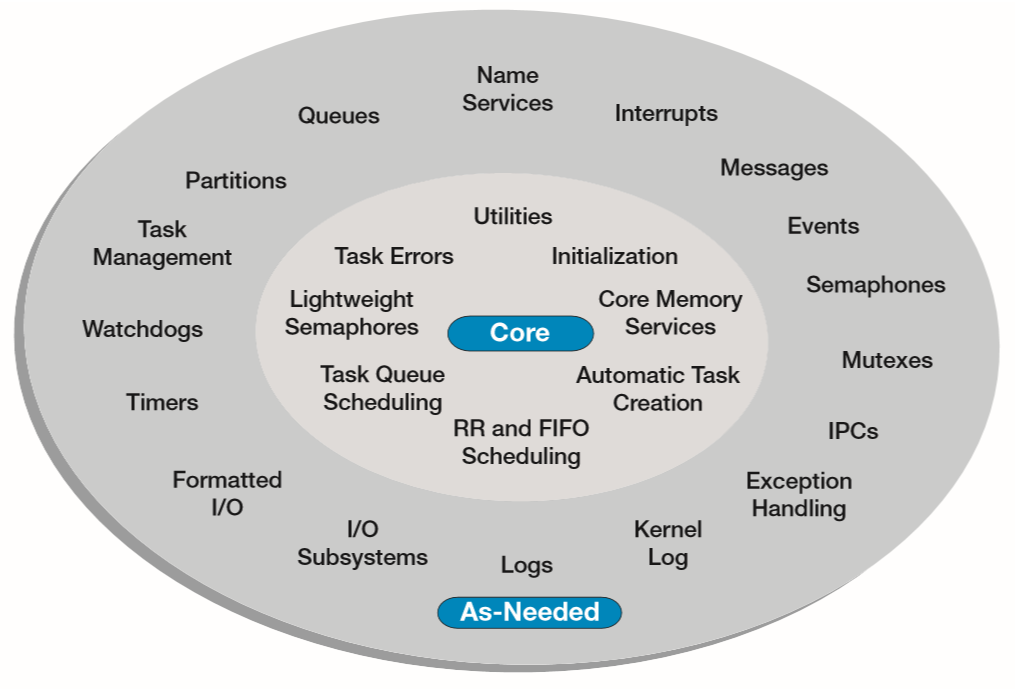
\includegraphics[width=\textwidth]{mqxBlocs}
\caption{Blocs personnalisables de MQX RTOS}
\end{figure}
La robustesse et la fiabilité de MQX RTOS donne une plateforme de confiance pour les applications critiques. MQX est certifié pour les applications médicales (\textsc{(cfr 820.30 part 21, iec 60601-1)} et aérospatiales \textsc{(do-178b)}. Les applications critiques de sécurité basé sur MQX comprennent l'équipement de chirurgie de l'œil, matériel d'injection de drogues, de l'équipement de surveillance de la dose de rayonnement, les systèmes de freinages des avions, et les équipements de navigation de l'avion.
\begin{figure}[H]
\centering
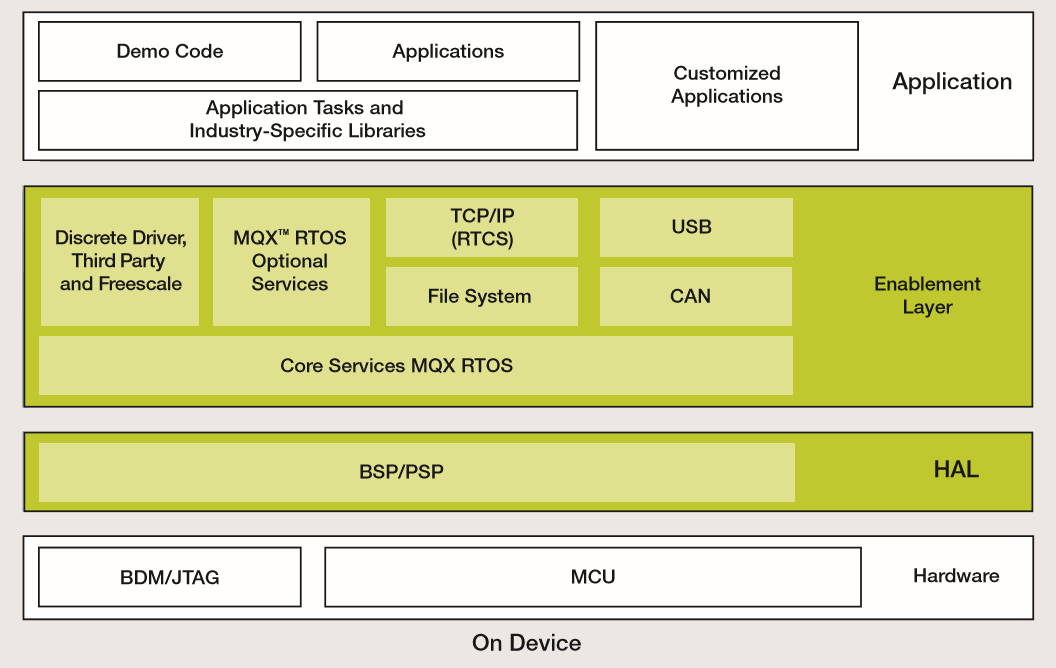
\includegraphics[width=\textwidth]{mqx}
\caption{Solution Freescale MQX}
\end{figure}
\section{Les tâches}
En utilisant le système d'exploitation MQX RTOS, tout ce qui reste à faire dans la partie programme est de créer des sous-programmes appelés les tâches. Ces tâches seront exécuté en parallèles par ordre de priorité en utilisant l'algorithme Round-Robin. Durant ce stage, je n'ai pas pu réaliser les programmes, par faute de temps. Mais, je vais présenter brièvement les tâches planifiés.
\subsection{Maximum Power Point Tracking (MPPT)}
C'est une tâche qui s'occupera de la maximisation de la puissance en utilisant l'algorithme P\&O. cette tâche sera exécuté périodiquement suivant un intervalle qui varie selon le changement de puissance. L'annexe \ref{apdx:MPPT} présente en détail l'algorithme de la MPPT.
\subsection{Régulation}
La tâche de la régulation consiste à maintenir la tension sinusoïdale de sortie à 220V. il s'occupera de la lecture de la tension de sortie, prendre une décision, et agir sur les signaux PWM.

\subsection{Communication}
La tâche de la communication va devoir s'occuper de trouver le serveur qui va stocker les informations collecté régulièrement. Ces informations seront éventuellement la puissance délivré par le panneau, la puissance absorbé par les charges, les valeurs de tensions et courant mesuré au fil du temps... Elle doit aussi exécuter des commandes délivré par le serveur qui seront défini ultérieurement.

\chapter*{Conclusion}
\addcontentsline{toc}{section}{Conclusion}
Lors de mon stage qui a duré deux mois à MAScIR, j'ai eu l'occasion de travailler sur le module communication du micro-onduleur. En commençant par l'étude et le choix du support de communication le mieux adapté pour ces types d'applications, la communication Ethernet et Power Line Communication s'avèrent les plus qualifiés pour un tel usage.\\

L'implémentation de la communication PLC commence par le choix d'un modulateur du signal, suivi d'un dimensionnement du circuit d'injection qui est composé de filtres de transmission et de réception et d'un montage d'isolation.
La communication Ethernet dans ce projet dépend fortement du microcontrôleur, par ce que le microcontrôleur choisi inclus les composants nécessaires pour ce type de communication.\\

La deuxième partie de mon stage était de regrouper la partie commande et communication en un seul circuit imprimé et en utilisant un seul microcontrôleur. Le travail a été surtout focalisé sur le choix idéal du microcontrôleur pour l'intégrer avec le reste des modules, et le design du circuit imprimé.\\

Parmi les difficultés rencontrées, l'insuffisance de deux mois pour développer les programmes, que ça soit du côté client (micro-onduleur) ou côté serveur.

\appendix
\chapter{CENELEC - EN 50065-1}
SIGNALLING ON LOW-VOLTAGE ELECTRICAL INSTALLATIONS IN THE FREQUENCY RANGE 3 KHZ TO 148,5 KHZ - PART 1: GENERAL REQUIREMENTS, FREQUENCY BANDS AND ELECTROMAGNETIC DISTURBANCES\\

\paragraph{Scope}
This standard applies to electrical equipment using signals in the frequency range 3 kHz to 148,5 kHz to transmit information on low voltage electrical systems, either on the public electricity distribution network or within installations in consumers' premises.\\

It specifies the frequency bands allocated to the different applications, limits for the terminal output voltage in the operating band and limits for conducted and radiated disturbance. It also gives the methods of measurement.\\

It does not specify the modulation methods, the coding methods or functional features (except those for the prevention of mutual interference).\\

Environmental requirements and tests are not included.\\

NOTE 1 Compliance with this standard does not imply permission to establish communication with locations outside the consumer's installation or with other consumers through the public electricity distribution network where this would not otherwise be allowed.\\

The object of the standard is to limit mutual influence between transmission equipment in electrical installations and between such equipment and other equipment. In addition this standard is intended to limit interference caused by signal transmission equipment to sensitive electronic equipment. However, complete freedom from such interference cannot be assured.\\

NOTE 2 Designers should consider signalling systems in conformance with this standard when determining immunity for electrical equipment.

\chapter{CSMA}
CSMA est l’acronyme de "\textbf{C}arrier \textbf{S}ense \textbf{M}ultiple \textbf{A}ccess" (Écoute d'un Support à Accès Multiple). Il s'agit d'un ensemble de protocoles d'accès à un média. Ceux-ci vérifient que le support est disponible avant de commencer l'envoi d'une trame. Ils permettent également de détecter ou bien éviter les collisions de messages dans les transmissions.\\

Pour éviter des erreurs lors de la transmission de données, il est nécessaire d'éviter les collisions. Cependant, selon le média et d'autres paramètres (débit, distance, codage...), il n'est pas possible d'utiliser une seule et unique méthode.\\

Il existe trois méthodes employées dans les réseaux :
\begin{itemize}
\item[CSMA/CD] : Collision Detection.
\item[CSMA/CA] : Collision Avoidance.
\item[CSMA/CR] : Collision Resolution (aussi appelé CSMA/BA pour "Bitwize Arbitration" ou CSMA/AMP pour "Arbitration on Message Priority").
\end{itemize}
Avant d'entrer dans la technique, il est utile pour une bonne compréhension de faire une analogie avec un groupe de personnes souhaitant discuter entre elles :\\

CSMA/CD correspond à un groupe dans lequel chaque personne peut prendre la parole quand elle le souhaite (lors d'un silence). Si deux personnes parlent en même temps, elles s'arrêtent et attendent un petit temps (aléatoire pour chaque personne).\\

CSMA/CA ressemble plus à un groupe d'élèves dans une classe : lorsqu'un élève veut parler, il doit lever la main et l'enseignant va l'autoriser à parler pour une durée définie. Si un élève au premier rang lève la main, il ne peut pas voir celui qui a levé également la main au fond, d'où l'importance du rôle de l'enseignant.\\

CSMA/CR sera plus difficile à imaginer : dans un groupe de personne, si deux personnes parlent en même temps, elles continuent de le faire tant qu'elle disent strictement la même chose. Dès que les paroles divergent, un arbitrage logique est fait et l'une des personnes s'arrête, laissant l'autre terminer sa phrase.

\paragraph*{CSMA/CD (Collision Detection)}
La méthode CSMA/CD (Carrier Sense Multiple Access / Collision Detection) est dérivée d'un système de transmission radio appelé Aloha. Son principe est de laisser chacun libre de gérer ses émissions en fonction de ses besoins et de la disponibilité du média.\\

En l'absence d'information à transmettre, la station écoute (ou reçoit) les paquets qui circulent sur le média dans un sens ou dans l'autre. Quand la station a besoin d'émettre un ou plusieurs paquets, elle vérifie qu'aucune trame n'est émise sur le média. Si c'est le cas elle commence à émettre son paquet. Si ce n'est pas le cas elle attend la fin de la transmission en cours. \\

Chaque machine ayant à tout instant la possibilité de commencer une transmission de manière autonome, la méthode d'accès est distribuée : elle est dite à accès multiple (Multiple Access : MA). La machine observe le média en cherchant à détecter une porteuse (Carrier Sense : CS). Si aucune trame n'est transmise, elle ne trouve pas de porteuse.\\

Elle envoie ses paquets sur le support physique et reste à l'écoute du résultat de son émission pendant quelque temps, pour vérifier qu'aucune autre machine n'a suivi le même comportement qu'elle au même instant.\\

La méthode d'accès étant à détection de collision (Collision Detect : CD), lors de son émission une machine peut déceler un problème de contention, et s'arrêter avec l'intention de renvoyer son paquet ultérieurement quand elle aura de nouveau la parole. De façon à minimiser le risque de rencontrer une deuxième collision avec la même machine, chacune attend pendant un délai aléatoire avant de tenter une nouvelle émission.\\

Cependant, de manière à ne pas saturer un réseau qui s'avérerait déjà très chargé, la machine n'essaiera pas indéfiniment de retransmettre un paquet si à chaque tentative elle se trouve en conflit avec une autre ; après un certain nombre d'essais infructueux (le nombre maximum de reprises est de 16) le paquet est éliminé. On évite ainsi l'effondrement du réseau. Les couches supérieures sont averties que la transmission du message a échoué.

\paragraph{CSMA/CA (Collision Avoidance)}
La méthode CSMA/CA s'utilise dans les réseaux sans-fil. En effet, contrairement aux réseaux filaires, deux stations peuvent émettre vers une troisième sans se détecter (la première étant hors de portée de la seconde).\\

Pour éviter cela, une station est considérée comme le maître des transmissions qui autorise une station à communiquer lorsque celle-ci le demande. Pour cela, la station doit émettre une courte trame RTS (Ready To Send) contenant quelques informations sur la communication (débit, longueur de la trame, etc.)\\

Si la station maître accepte cette communication, elle renvoie alors une trame CTS (Clear To Send) et la station peut transmettre son message. En revanche, si la station ne reçoit pas de message elle doit attendre à nouveau avant de redemander une autorisation d'émettre.\\

C'est la méthode utilisée dans les réseaux WiFi (802.11) et la station maître est généralement le point d'accès (AP).

\paragraph{CSMA/CR (Collision Resolution)}
Cette méthode est légèrement plus évoluée que la méthode CSMA/CD : si plusieurs stations transmettent un message, elles appliquent un ET logique entre le signal reçu et le signal émis. Dans le cas d'une inégalité, la station s'arrête de transmettre. Comme le 0 est une valeur dominante, elle écrase donc le 1 (état récessif) : cela signifie que la communication de l'une des stations n'est pas modifiée et permet ainsi de terminer cette communication sans délai d'attente ou de retransmission.\\

Un réseau utilisant cette méthode peut alors être déterministe. C'est la méthode employée dans les réseaux CAN.

\chapter{Description de MPPT}
\label{apdx:MPPT}
La puissance de sortie en courant continu provenant du panneau solaire est périodiquement calculée à l'aide de l'algorithme P\&O pour MPPT.\\

Cette méthode est basée sur l'algorithme simple et efficace P\&O. Dans le point d'une puissance P1, vous pouvez essayer d'avoir une puissance supérieure du panneau solaire en augmentant le courant à partir du panneau. Cela donne un nouveau point de puissance P2.
La nouvelle puissance actuelle est calculée par le produit de la tension d'entrée et le courant d'entrée. Cette valeur est comparée avec la valeur échantillonnée précédente.
Si la nouvelle valeur de puissance est supérieure à la valeur précédente, la puissance d'entrée augmente. Ainsi, la direction de déplacement de la courbe de puissance est correcte.
Dans l'étape suivante, vous pouvez essayer de couler courant encore plus élevé à partir du panneau. La mesure de puissance dans le nouveau point peut être P3 en comparaison avec la valeur précédente.
La prochaine étape est analogique — c'est dans le cas où la puissance de sortie du panneau solaire est plus faible (Pn) — Retournez et essayer de trouver le point où la puissance provenant du panneau est la plus élevée.
Les flèches de la figure \ref{fig:mppt}} montrent la direction de déplacement du nouveau point de puissance. Le pas d'incrémentation dépend du changement de la puissance à l'étape précédente. Si la variation de puissance est plus élevée, le pas suivante est plus élevée. Si la variation de puissance est plus faible, le pas de la prise de courant est également plus petit suivant.
La puissance en haut de la courbe (dans le point Pmax) est horizontalement plat. Cela signifie que la variation de puissance est faible et la variation du pas est également faible. Ainsi, le point de puissance maximale est prise très précis. La fréquence de la vérification de la puissance délivrée par le panneau solaire doit être suffisamment élevée pour suivre correctement le MPP lorsque les conditions d'éclairage sont rapidement changées.
\begin{figure}[h]
\label{fig:mppt}
\centering
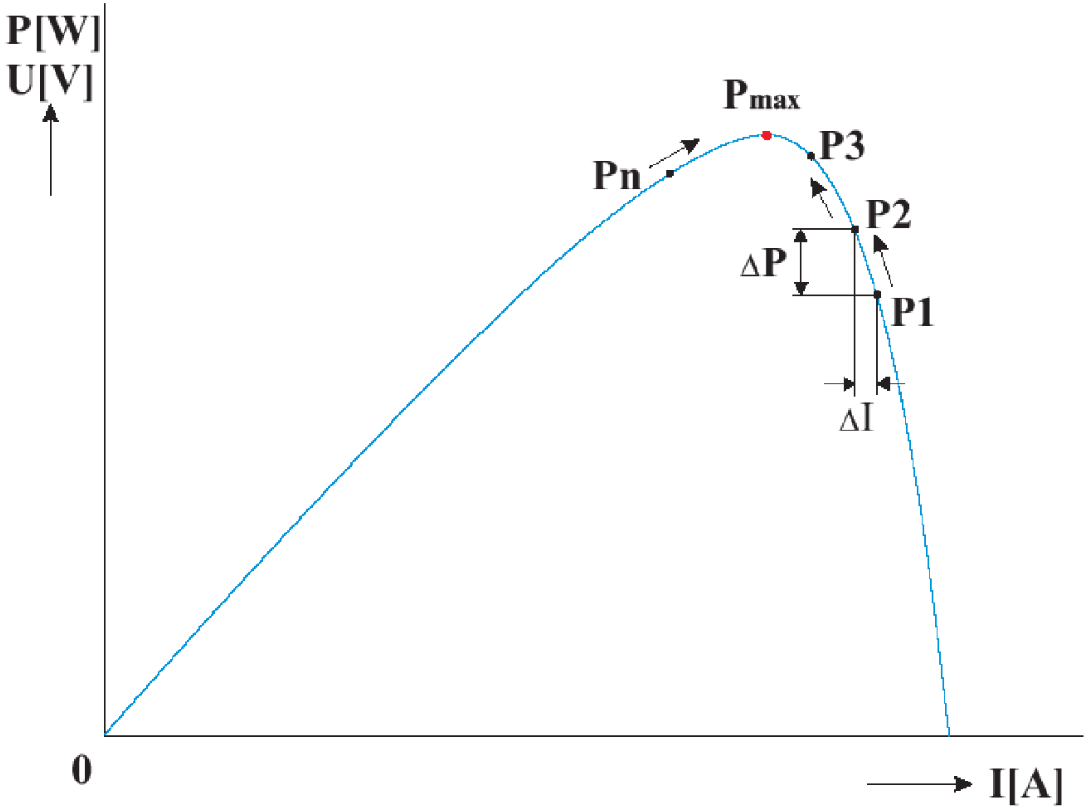
\includegraphics[width=\textwidth]{mppt}
\caption{l'algorithme MPPT}
\end{figure}

\chapter{Schéma du Daughter-card}
%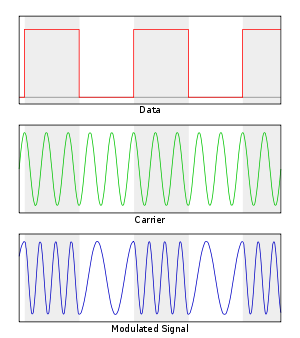
\includepdf[pages=1,landscape]{fsk.pdf}
%\includepdf[pages=1,landscape]{mcu.pdf}

\chapter{Schéma du circuit imprimé}
%\includepdf[pages=3,landscape]{Inverter_daughterCard.pdf}
\begin{figure}[h]
\centering
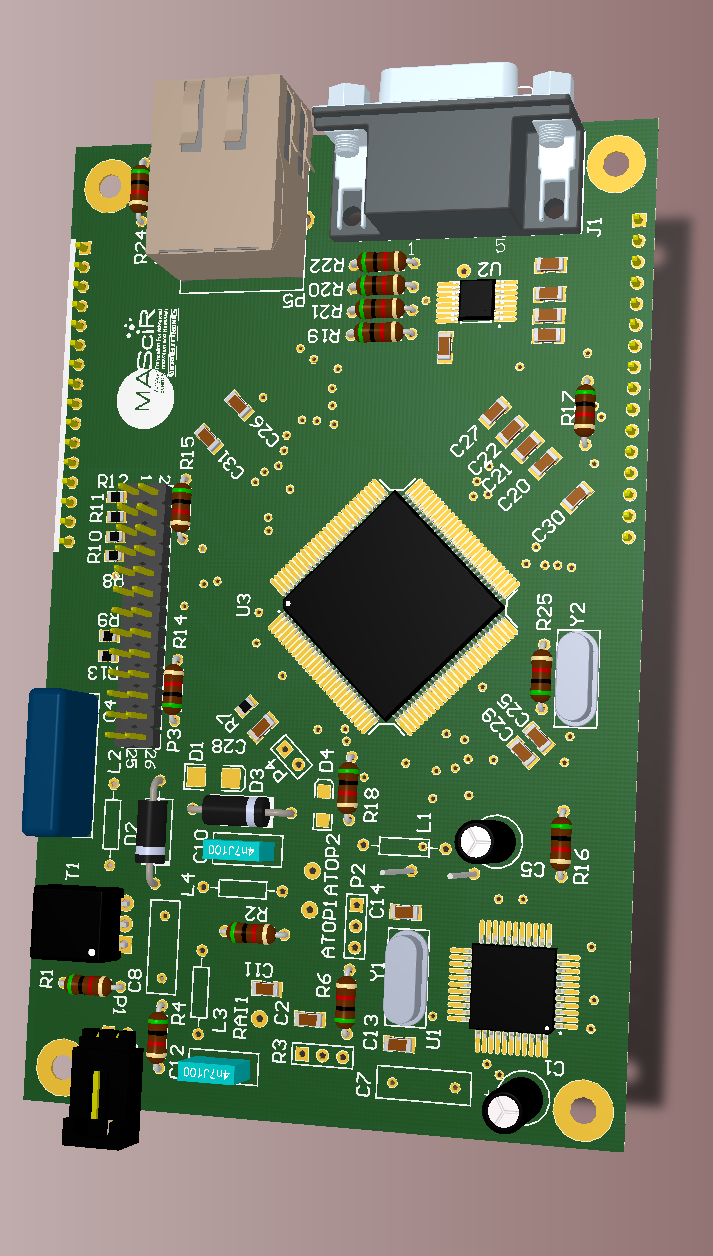
\includegraphics[width=\textwidth]{pcb}
\end{figure}

\begin{thebibliography}{9}
  
\bibitem{plc}
  (fr)
  Etienne DURIS, Loïc Heuzé, Woollams Kwame, Zidouri Hakima,
  \emph{Courants porteurs en ligne},
  Universié Paris-Est Marne-la-Vallée(UPEM),
  Février 2005.\\
  
\bibitem{st7538q}
  (en)
  ST Microelectronics,
  \emph{ST7538Q},
  Datasheet, Rev 1, July 2006.\\
  
\bibitem{cenelec}
  (en)
  European Committee for Electrotechnical Standardization,
  \emph{Standard: CENELEC - EN 50065-1},
  April 01, 2011.\\

\bibitem{anst7538q}
  (en)
  ST Microelectronics,
  \emph{ST7538Q FSK powerline transceiver demonstration kit description},
  Application note, Rev 4, February 2008.\\
  
\bibitem{ansp}
  (en)
  Freescale Semiconductor,
  \emph{Inverter for the Solar Panel using an MC56F8023},
  Application note, Rev 0, September 2011.\\
  
\bibitem{mcf52235}
  (en)
  Freescale Semiconductor,
  \emph{MCF52235},
  Datasheet, Rev 10, March 2011.\\
  
\bibitem{mcf52233DEMO}
  (en)
  Axiom Manufacturing,
  \emph{MCF52235 AXM-0384},
  Schematics, Rev E1.\\
  
\bibitem{mqx}
  (en)
  Freescale Semiconductor,
  \emph{Freescale MQX™  Software Solutions, Complimentary proven RTOS, TCP/IP,  file system and USB},
  Fact Sheet, Rev 10.\\

\end{thebibliography}

\end{document}